\chapter{Étude technique}
\label{chap:technique}
Ce chapitre est consacré à l'étude technique réalisée pour la mise en œuvre du projet. En
abordant les besoins techniques, la définition de l'architecture technique du système, et en
présentant par la suite les technologies et les outils utilisés dans la phase de réalisation. Et en
clôturant par l'illustration des environnements matériels et logiciels utilisés dans le projet ainsi
que les outils définis pour supporter la méthodologie de travail.

%------------------------------------------------------------
\section{Architecture du projet}
Dans le contexte du développement logiciel, l'architecture d'un projet se réfère à la structure et à
l'organisation des principaux composants du système, ainsi qu'à la manière dont ils interagissent
entre eux. Elle englobe divers aspects, tels que la stratégie commerciale, les attributs de qualité,
la dynamique humaine, la conception et l'environnement informatique.

\subsection{Architecture physique}

L'architecture technique du système LMS repose sur une infrastructure moderne et scalable, conçue pour supporter les exigences des fiduciaires belges. Notre solution combine robustesse et flexibilité grâce aux composants suivants :

\begin{table}[htbp]
\centering
\begin{tabular}{|p{3cm}|p{10cm}|}
\hline
\textbf{Composant} & \textbf{Valeur ajoutée} \\ \hline
\textbf{Git} & Versionnement précis avec historique complet des évolutions \\ \hline
\textbf{GitHub Actions} & Automatisation des tests et déploiements après chaque modification \\ \hline
\textbf{PHP-FPM 8.2} & Exécution performante du code métier avec gestion optimisée des ressources \\ \hline
\textbf{Nginx} & Serveur web haute performance avec gestion intelligente du cache \\ \hline
\textbf{MySQL 8} & Stockage relationnel des données avec transactions ACID \\ \hline
\end{tabular}
\end{table}

\begin{figure}[htbp]
\centering
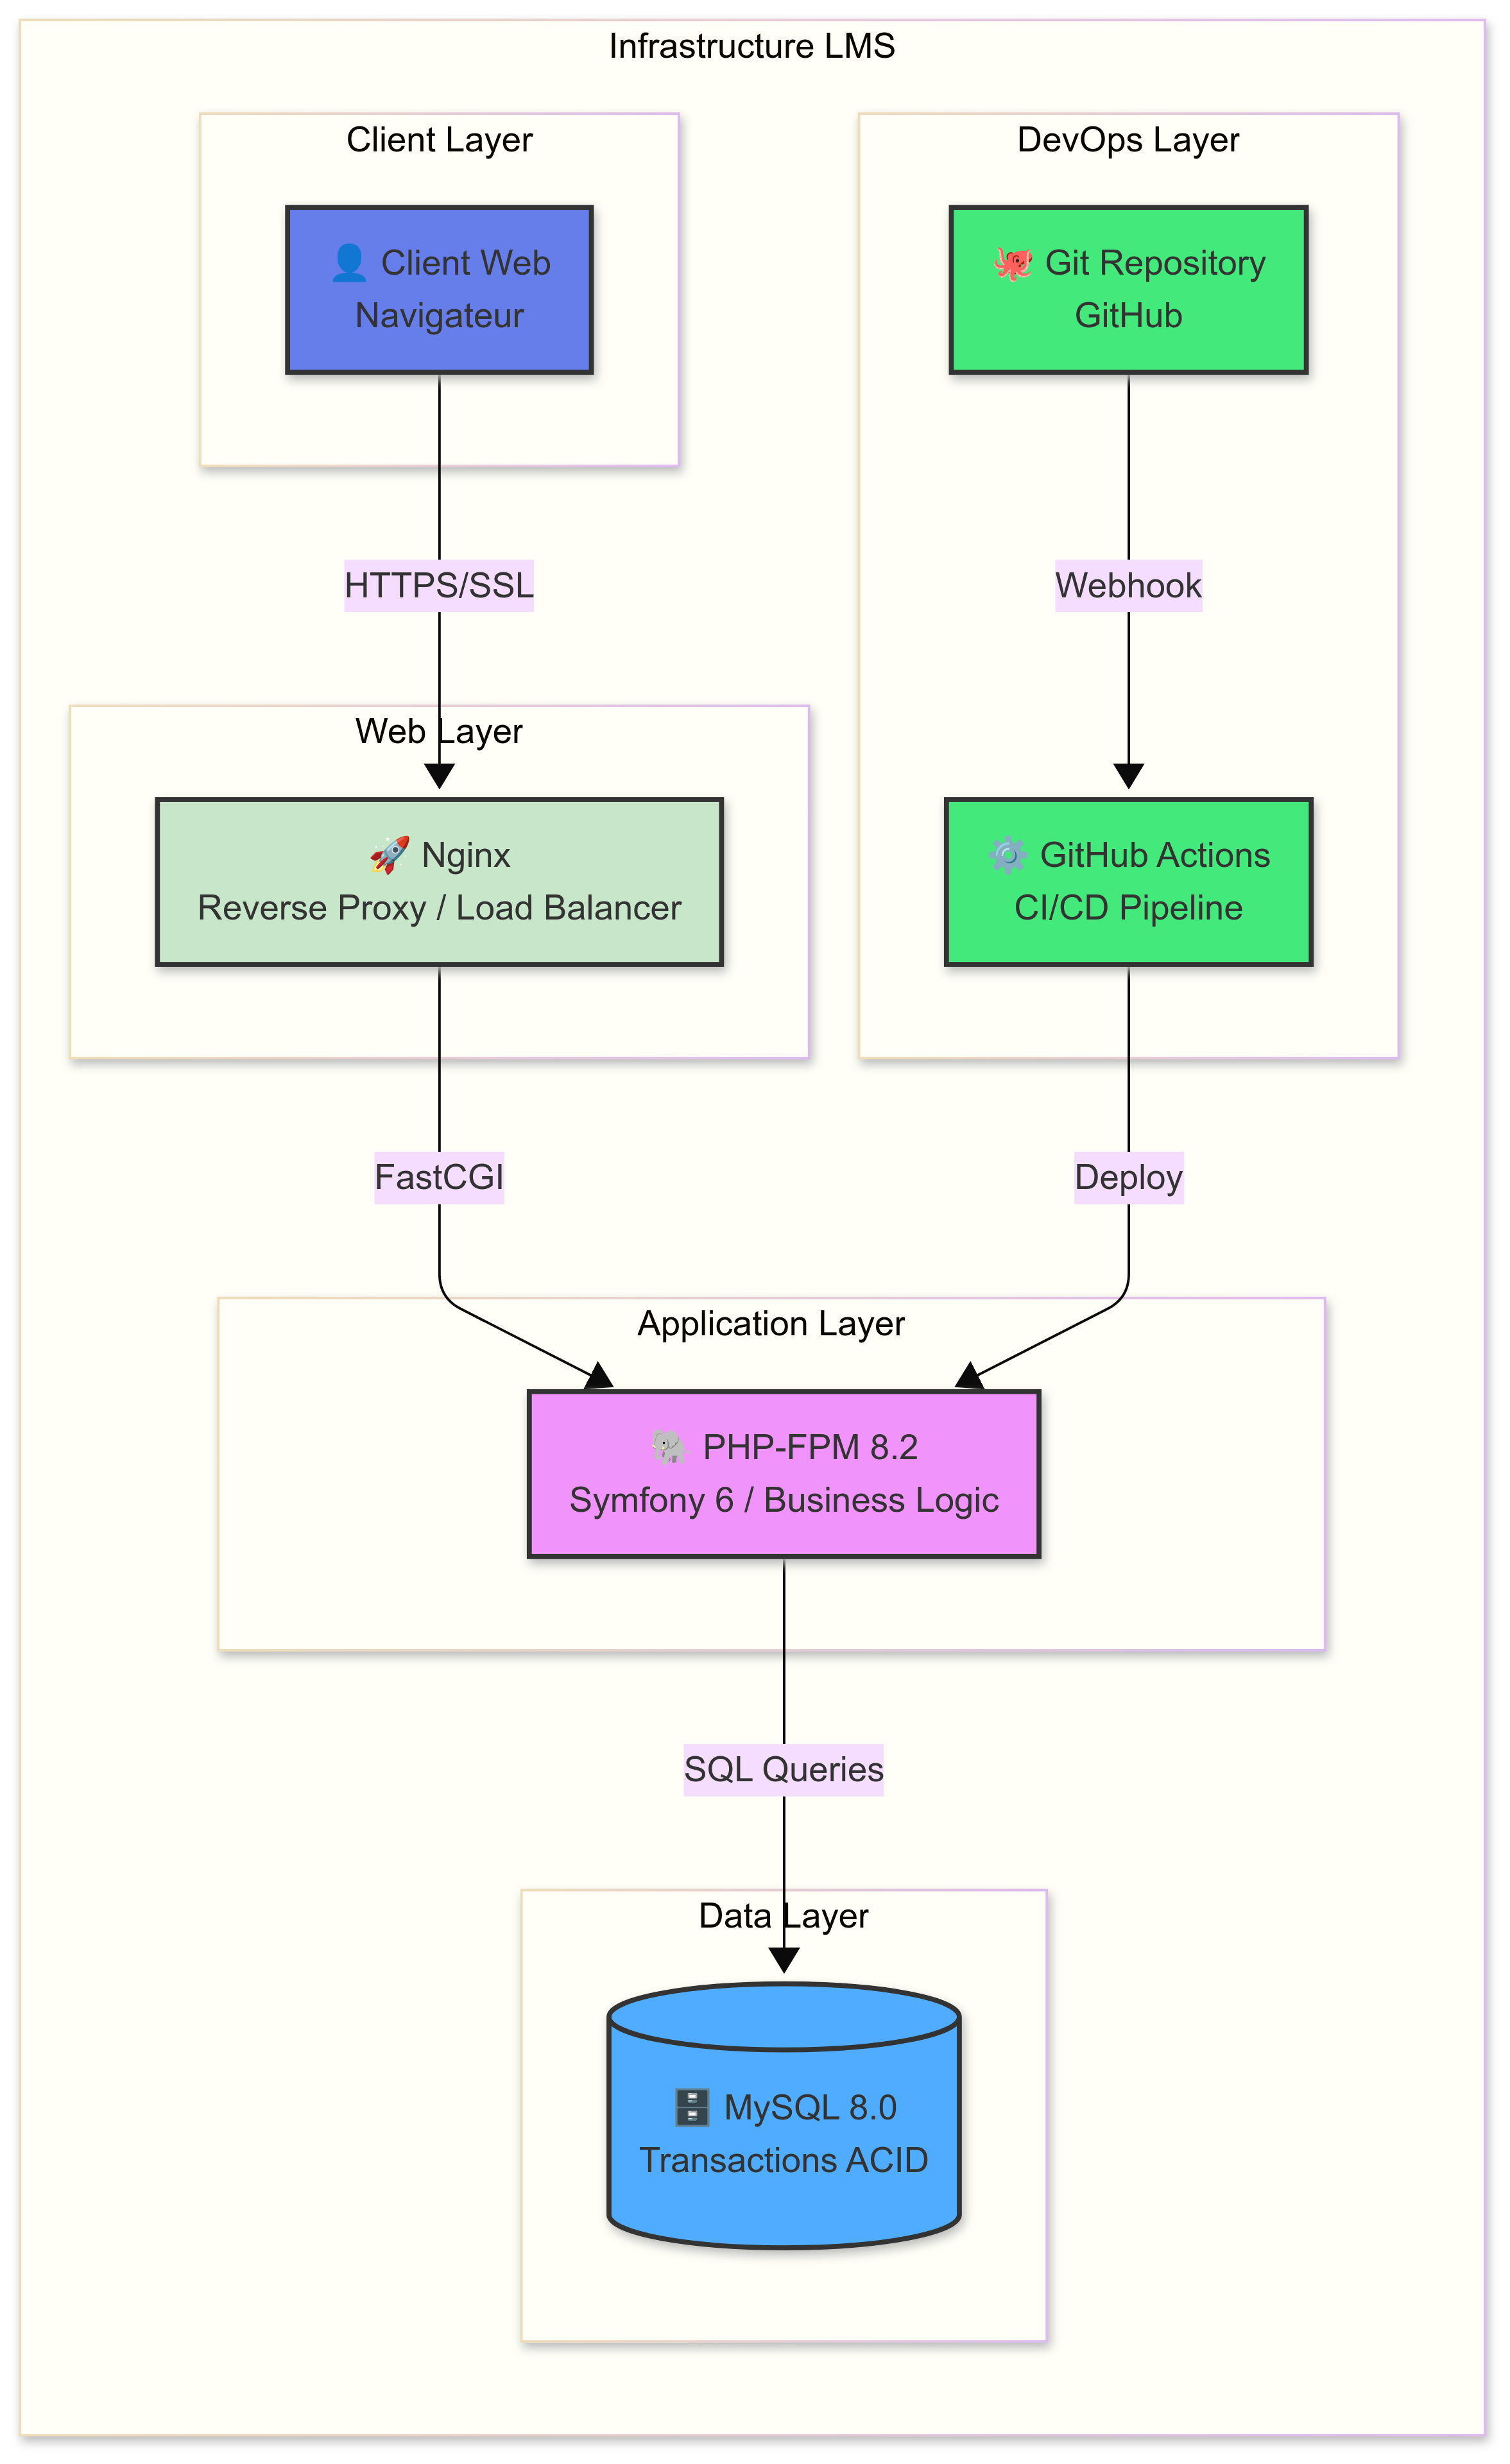
\includegraphics[width=0.8\linewidth]{lmsstructure.png}
\caption{Architecture technique du système Webinar Didier}
\label{fig:archi-tech}
\end{figure}
\newpage

\subsection{Architecture logique}
L'architecture logique décrit comment le code est organisé ainsi que les standards de
programmation suivis au sein de l'environnement TAMTAM.

\subsubsection{Modèle MVC amélioré}
Notre implémentation du pattern MVC intègre des bonnes pratiques spécifiques au contexte LMS :

\begin{figure}[ht!]
\centering
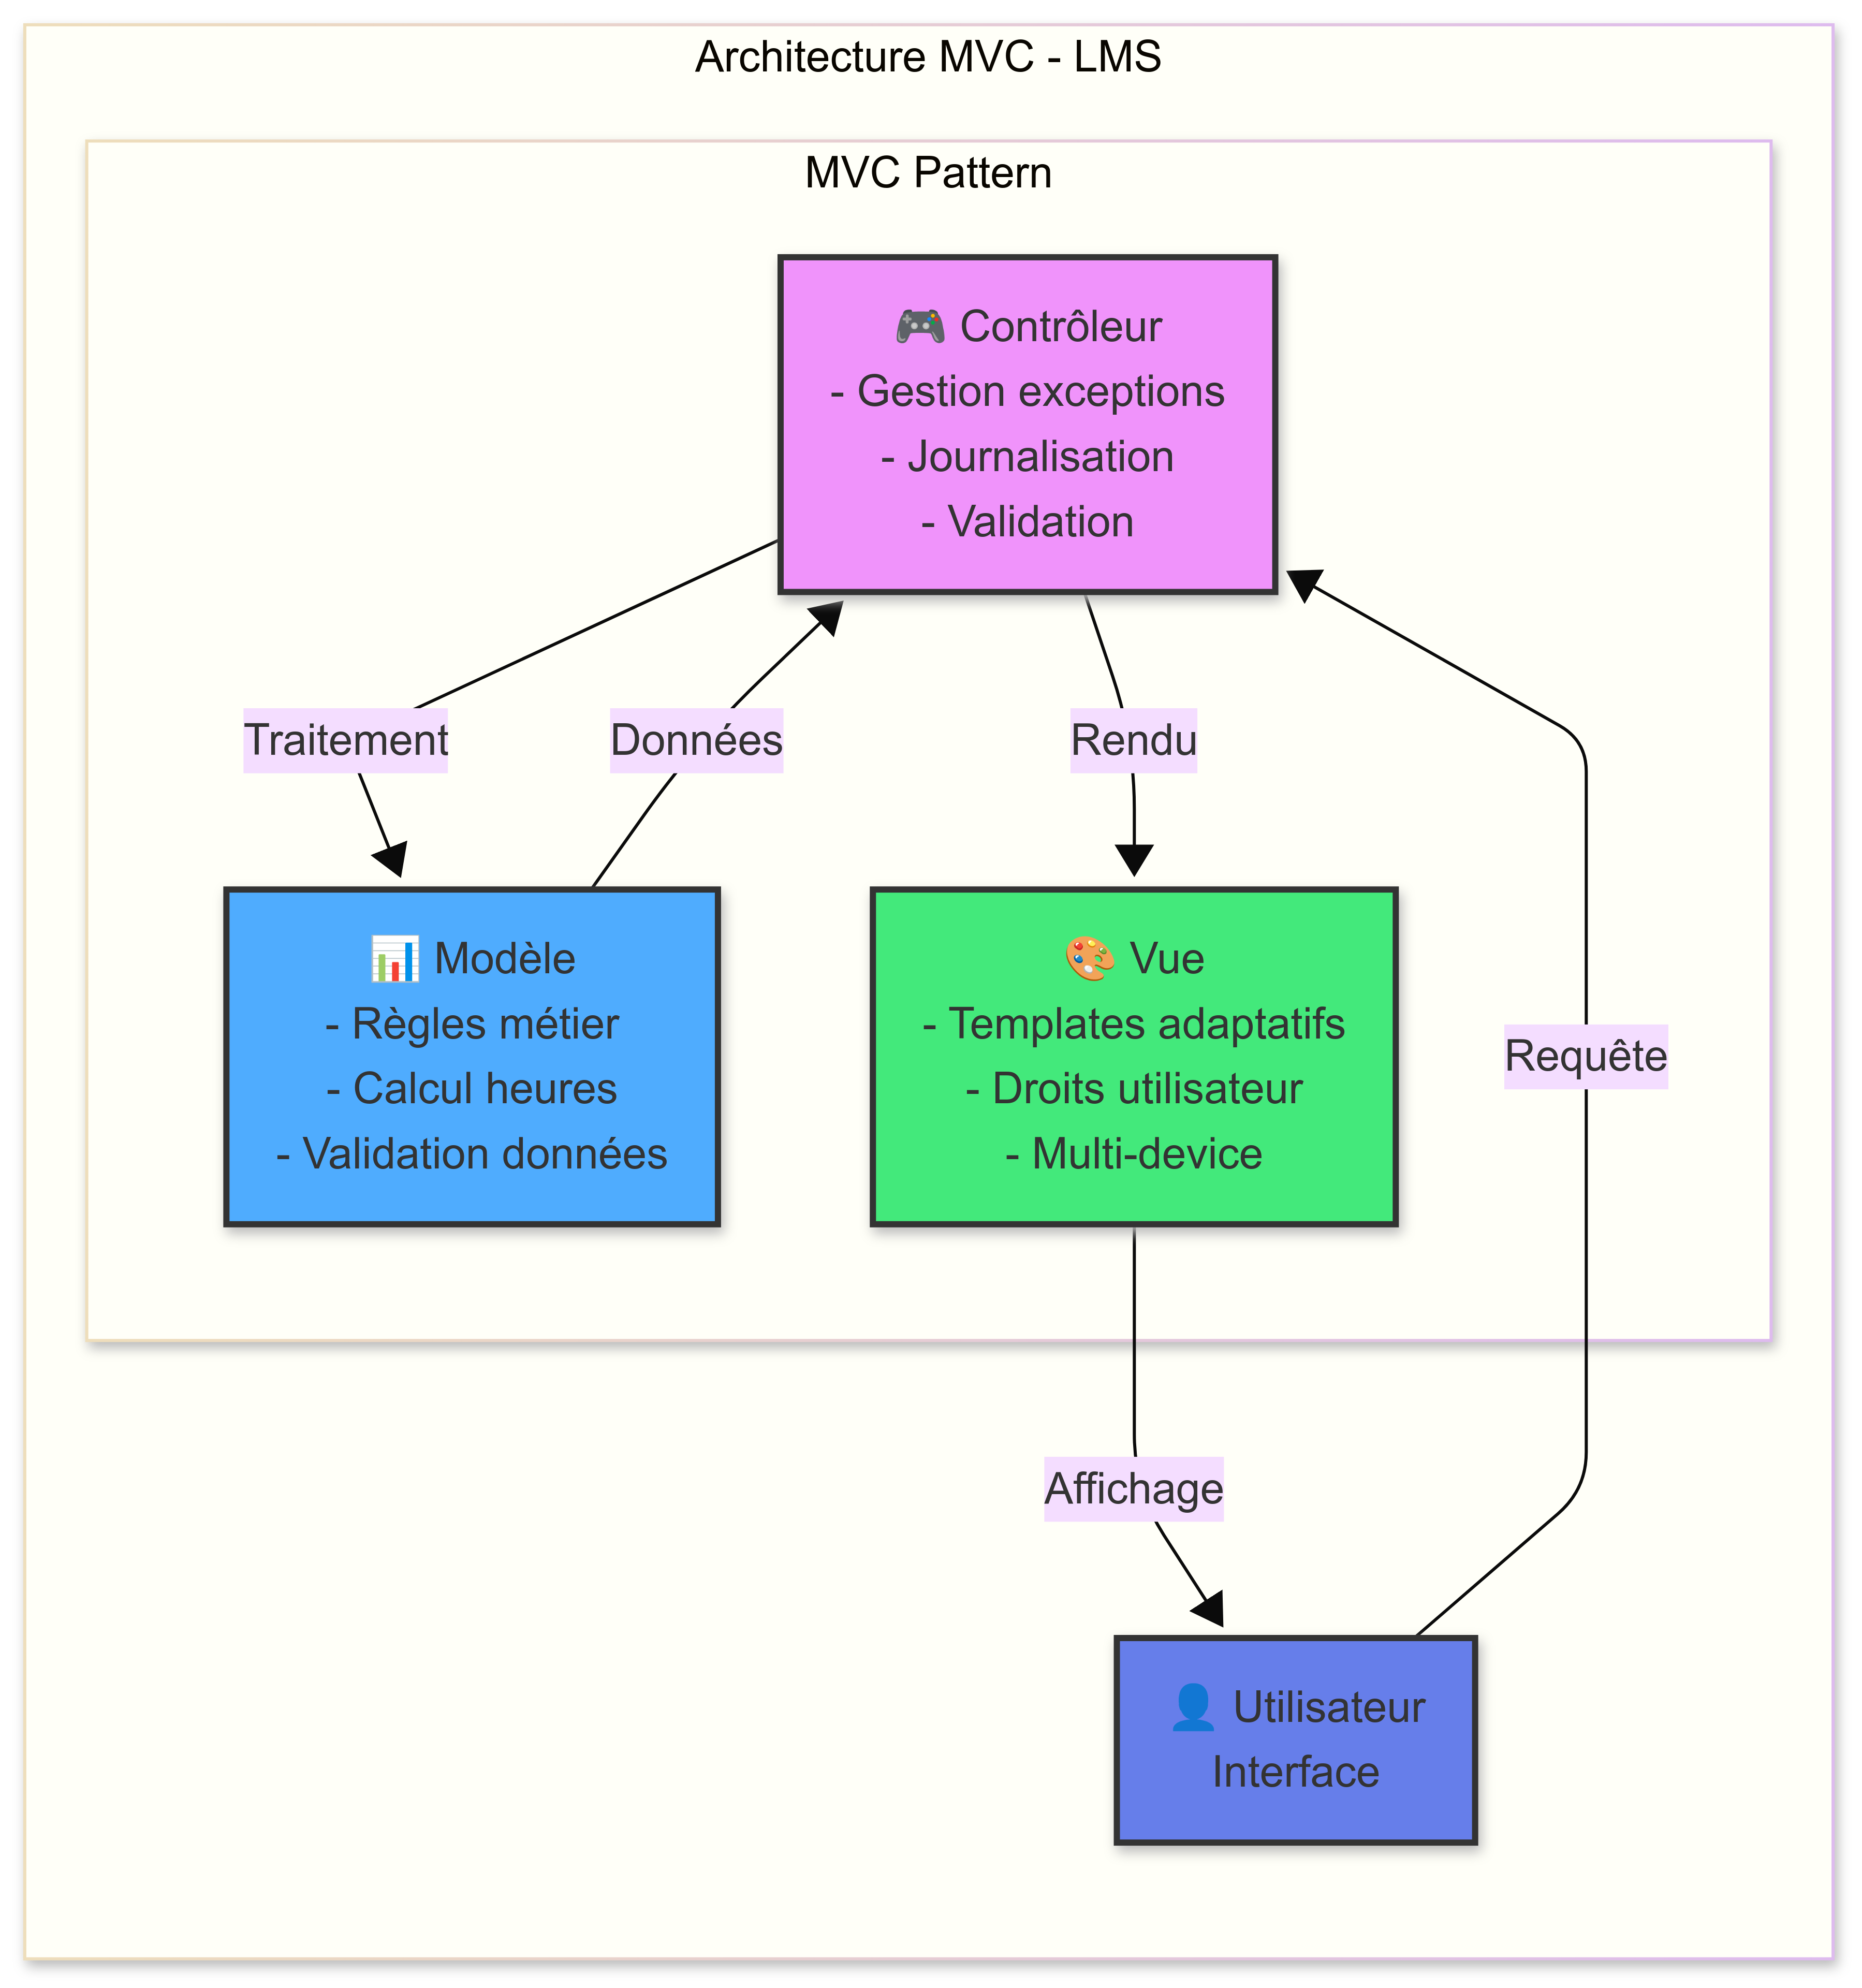
\includegraphics[width=1\linewidth]{mvc.png}
\caption{Flow MVC adapté pour le LMS}
\label{fig:mvc-flow}
\end{figure}

\begin{itemize}
\item \textbf{Modèle} :
\begin{itemize}
\item Couche métier enrichie pour gérer les règles complexes de calcul des heures de formation
\item Validation stricte des données pédagogiques
\end{itemize}
\item \textbf{Vue} :
\begin{itemize}
\item Génération dynamique des interfaces en fonction des droits utilisateur
\item Templates adaptatifs pour différents devices
\end{itemize}
\item \textbf{Contrôleur} :
\begin{itemize}
\item Gestion centralisée des exceptions métier
\item Journalisation détaillée des actions sensibles
\end{itemize}
\end{itemize}

\subsubsection{Structure du projet}
Nous avons conçu l'architecture de notre projet en respectant l'architecture logique établie lors de l'étude technique. Notre application est divisée en deux parties : côté Back-end et côté Front-end. Nous allons présenter les dossiers et les répertoires du projet ainsi que leurs fonctionnalités par rapport à l'objectif du projet LMS.

\paragraph{Architecture logique complète}
La structure du projet LMS s'articule autour d'une architecture modulaire qui sépare clairement les responsabilités entre le back-end et le front-end, tout en maintenant une cohésion fonctionnelle optimale.

\begin{figure}[htbp]
\centering
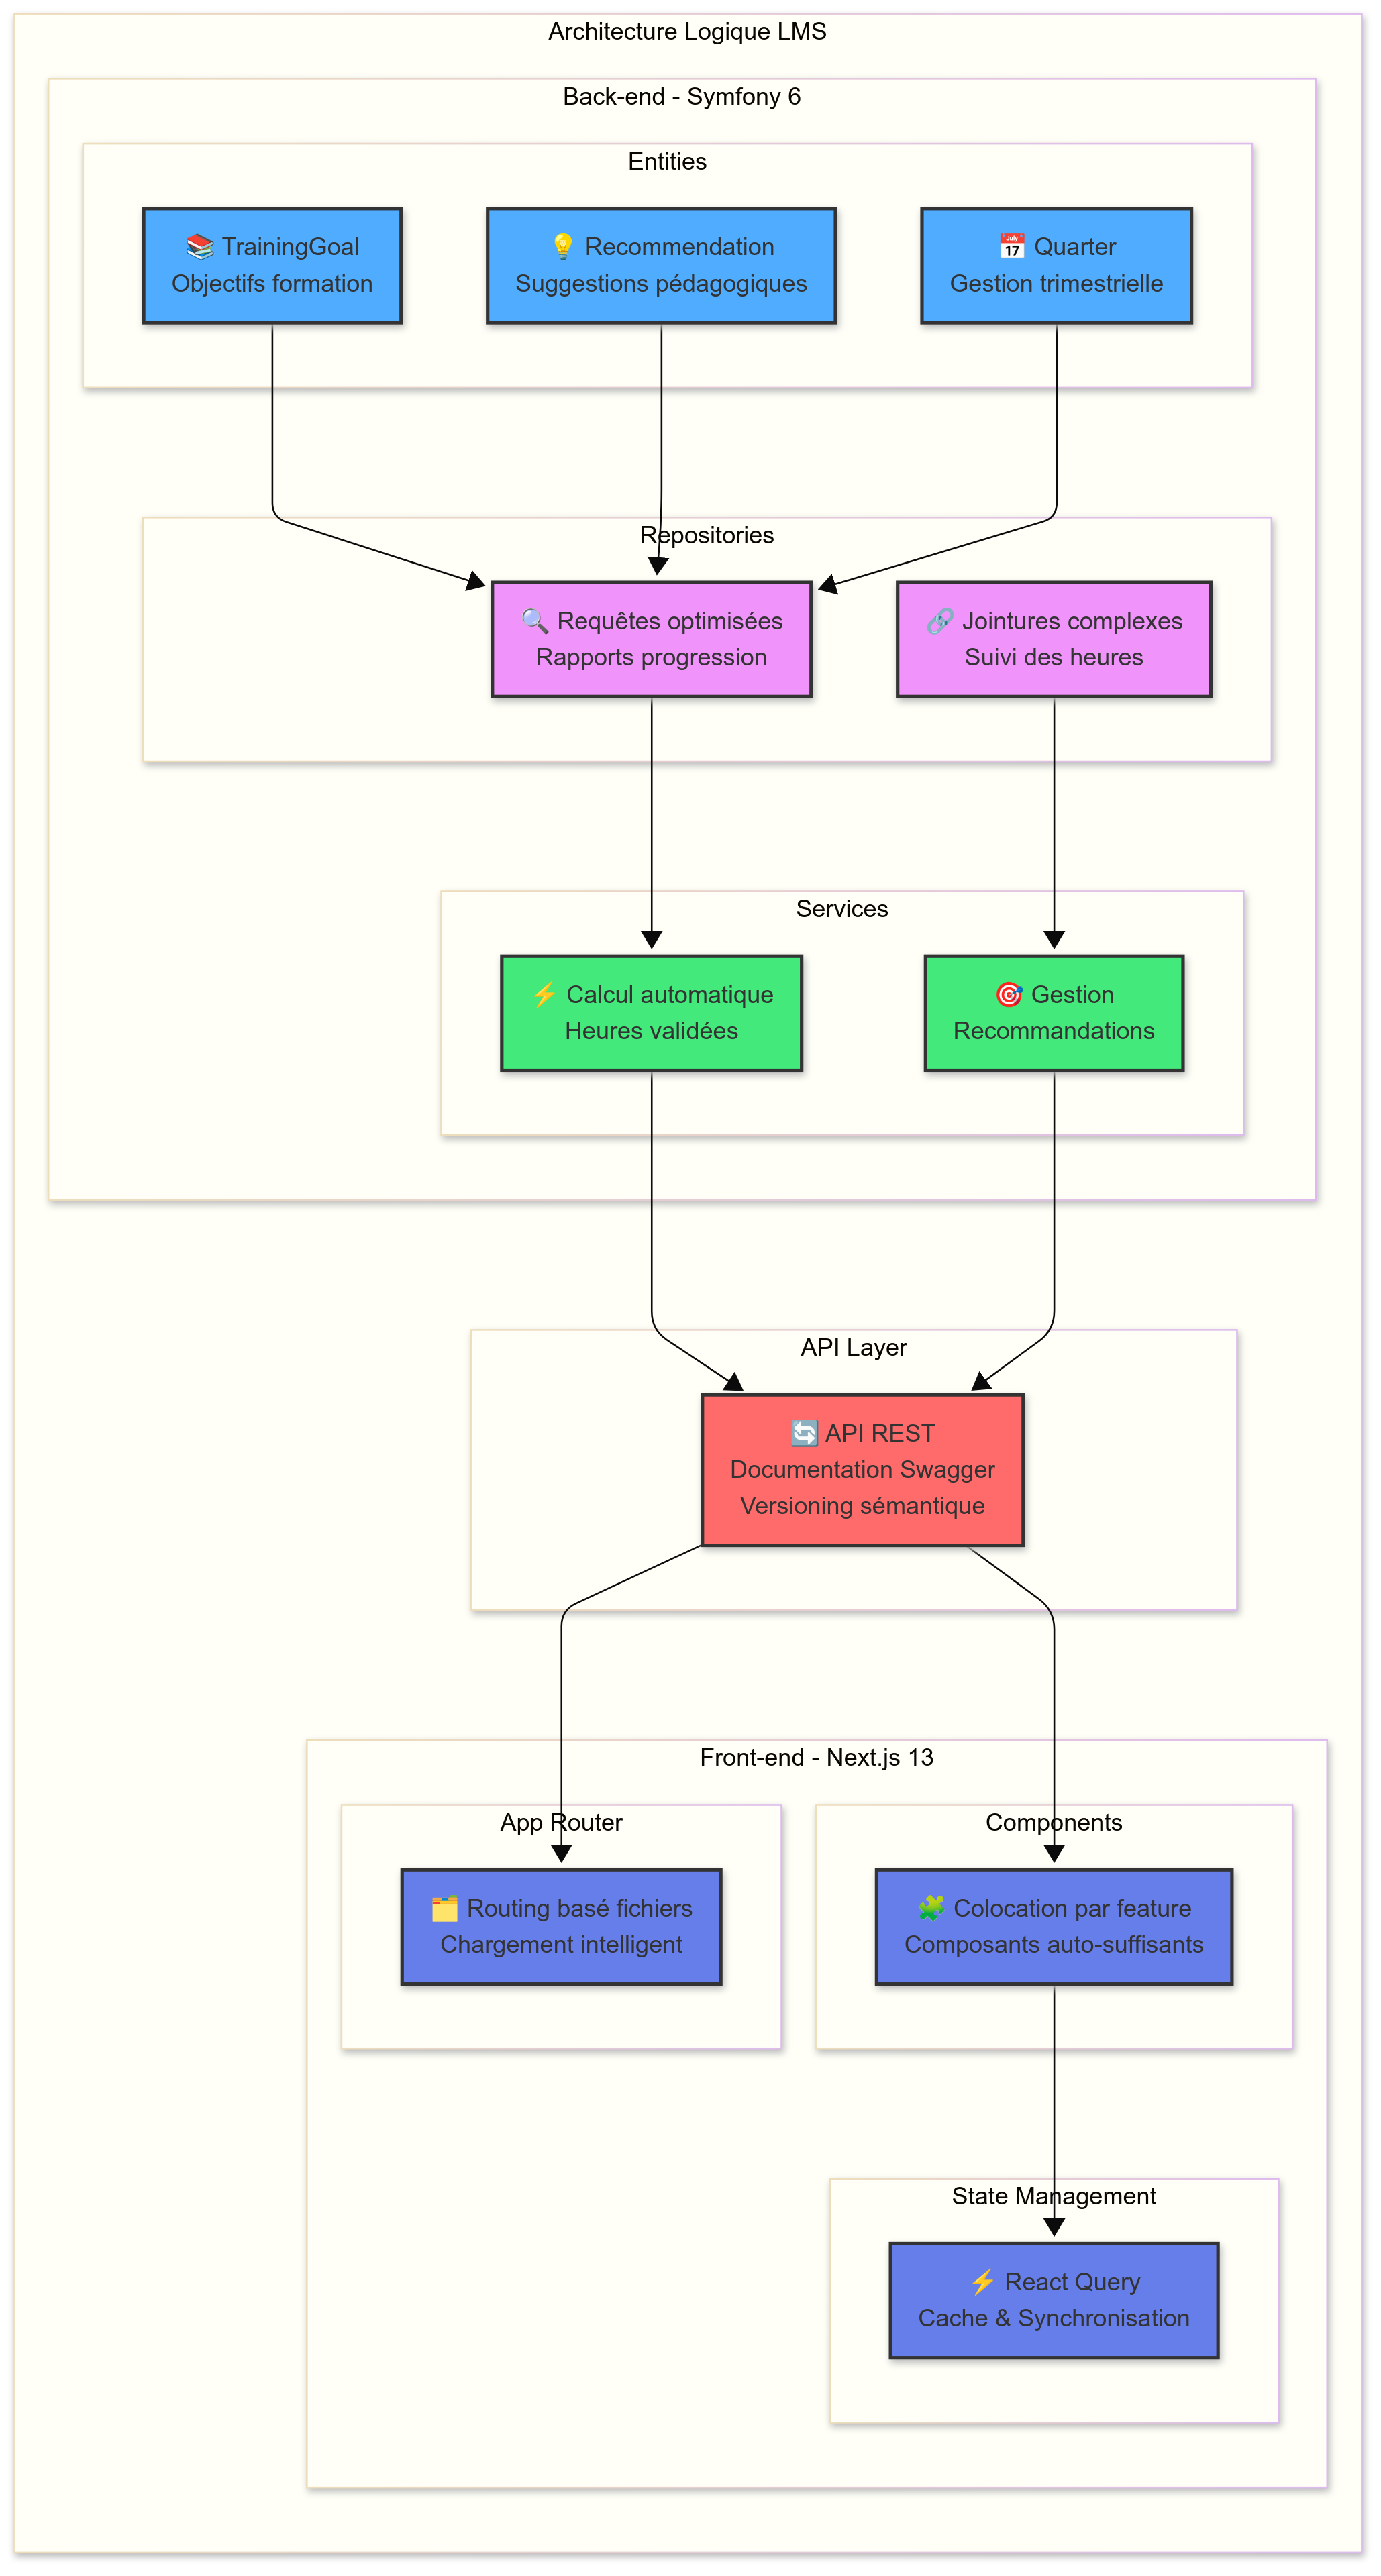
\includegraphics[width=0.8\linewidth]{logique.png}
\caption{Structure logique du projet LMS}
\label{fig:structure-projet}
\end{figure}
\newpage

\paragraph{Côté Back-end}
La partie back-end est centralisée dans une grande API qui contient plusieurs bundles. Chaque projet TAMTAM se représente par un bundle, ce dernier étant un ensemble de fichiers et de répertoires permettant d'implémenter les fonctionnalités d'une application précise. Dans le cas de ce projet, le back-end est représenté par le \texttt{EventBundle} situé sous le dossier \texttt{src/TTP}.

Voici une description de quelques dossiers du Bundle EventBundle :

\begin{itemize}
\item \textbf{Repository} : Contient les requêtes avec jointures complexes, réutilisables pour éviter les duplications de code.
\item \textbf{Resources} : Contient plusieurs fichiers de configuration de l'application en format YAML.
\item \textbf{Controller} : Gère les requêtes HTTP et coordonne les interactions entre les différentes couches de l'application.
\item \textbf{Service} : Un objet PHP remplissant une ou plusieurs fonctions associées à une configuration.
\item \textbf{Entity} : Contient toutes les entités du projet, c'est-à-dire les tables de la base de données.
\item \textbf{Event} : Contient tous les événements déclenchés selon les actions de l'utilisateur.
\item \textbf{Utils} : Classes utilitaires avec des méthodes prédéfinies réutilisables.
\item \textbf{Tests} : Tests fonctionnels et unitaires, ainsi qu'un dossier DataFixtures pour les données de test.
\item \textbf{Validator} : Validation des attributs des entités, par filtrage ou par rôle.
\end{itemize}

Entités principales dans le système LMS :
\begin{itemize}
\item \texttt{TrainingGoal} — Objectifs de formation
\item \texttt{Recommendation} — Suggestions pédagogiques
\item \texttt{Quarter} — Périodes trimestrielles
\end{itemize}

\paragraph{Côté Front-end}
Notre projet Next.js 13.4 adopte l'approche de colocation pour s'aligner avec la nouvelle architecture Next.js. Nous utilisons la convention \texttt{kebab-case} pour nommer les fichiers et dossiers, et travaillons avec TypeScript.

La structure de dossiers du projet est la suivante :
\begin{itemize}
\item \textbf{src/} : dossier racine de l'application.
\item \textbf{src/app/[lang]/feature/} : code d'une fonctionnalité (page, composants, hooks, services, constantes, types).
\item \textbf{src/app/[lang]/feature/page.tsx} : point d'entrée de la page.
\item \textbf{src/app/[lang]/feature/components/} : composants propres à la fonctionnalité.
\item \textbf{src/common/} : éléments partagés (components, services, constants, types, styles).
\item \textbf{src/common/services/misc/fetch-api-wrapper.ts} : wrapper d'appels API communs.
\item \textbf{src/common/constants/routes.ts} : définition centralisée des routes.
\item \textbf{src/contexts/} : providers de contexte.
\item \textbf{src/i18n/} : internationalisation et localisation.
\item \textbf{src/middleware.ts} : logique middleware (authentification, autorisation, redirections).
\end{itemize}

%------------------------------------------------------------
\section{Qualité de code}

\subsection{Outils de linting}
Nous appliquons une discipline stricte de qualité de code avec :
\begin{itemize}
\item \textbf{ESLint} : Configuration personnalisée basée sur Airbnb, détection des patterns problématiques, règles TypeScript strictes.
\item \textbf{Prettier} : Formatage automatique du code avec configuration partagée en équipe.
\item \textbf{Stylelint} : Cohérence CSS/SCSS et bonnes pratiques de style.
\end{itemize}

\subsection{Git Hooks}
Automatisation des vérifications via Husky :
\begin{itemize}
\item \textbf{pre-commit} : Exécution de lint-staged et vérification des types TypeScript.
\item \textbf{commit-msg} : Validation du format Conventional Commits. Exemple : \texttt{feat(lms): ajout calcul heures trimestrielles}.
\item \textbf{pre-push} : Exécution des tests unitaires et vérification de la build.
\end{itemize}

\subsection{Conventional Commits}
Standardisation des messages de commit :

\begin{longtable}{|l|p{10cm}|}
\hline
\textbf{Type} & \textbf{Usage} \\ \hline
\texttt{feat} & Nouvelle fonctionnalité \\ \hline
\texttt{fix} & Correction de bug \\ \hline
\texttt{docs} & Modification de documentation \\ \hline
\texttt{style} & Changement de formatage \\ \hline
\texttt{refactor} & Modification de code sans impact fonctionnel \\ \hline
\texttt{perf} & Amélioration de performance \\ \hline
\texttt{test} & Ajout ou modification de tests \\ \hline
\texttt{chore} & Tâches de maintenance \\ \hline
\end{longtable}

%------------------------------------------------------------
\section{Spécification technologique}
Pour décrire les spécifications technologiques de notre application, nous allons présenter les
technologies utilisées dans le développement.

\subsection{Outils de développement}

% ==============================================================
% MACRO : logo à gauche + titre + texte à droite (style image)
% ==============================================================
\newcommand{\techitem}[4][l]{%
\noindent
\begin{minipage}[t]{0.18\textwidth}
    \raggedright
    \vspace{0pt}
    \includegraphics[width=0.90\linewidth]{#2}\\[4pt]
    {\small\textit{Figure : logo #3}}
\end{minipage}%
\hspace{0.04\textwidth}%
\begin{minipage}[t]{0.75\textwidth}
    \vspace{0pt}
    {\large $\clubsuit$ \quad \textbf{#3 :}}\\[6pt]
    #4
\end{minipage}
\vspace{1.2em}
}

% ---- Node.js ----
\techitem{Chapters/img/nodejs.png}{Node.JS}{%
Node.js est \underline{une plateforme de développement JavaScript intégrant un serveur HTTP}.
Son fonctionnement se base sur une boucle événementielle qui lui permet le support de fortes montées en charge.
Dans notre projet, Node.js est utilisé pour bâtir des APIs légères, des services en temps réel
et des outils d'automatisation (scripts, watchers, serveurs de développement).%
}

% ---- React.js ----
\techitem{Chapters/img/react.png}{React.js}{%
React.js est une bibliothèque JavaScript dédiée à la construction d'interfaces utilisateur réactives et modulaires.
Son modèle basé sur les composants favorise la réutilisabilité et la maintenabilité du code front-end.
Dans notre contexte Webinar, il facilite la conception d'écrans interactifs et la gestion d'états complexes
via le Virtual DOM.%
}

% ---- Meteor.js ----
\techitem{Chapters/img/metor.png}{Meteor.js}{%
Meteor.js est une plateforme JavaScript full-stack qui simplifie le développement d'applications en temps réel.
Elle fournit un environnement unifié client/serveur et utilise le protocole DDP pour la synchronisation des données.
Dans le cadre du LMS, Meteor est utilisé pour les fonctionnalités collaboratives en temps réel
(chat, notifications, synchronisation d'état).%
}

% ---- Symfony ----
\techitem{logos/symfony.png}{Symfony Framework}{%
Symfony est un framework PHP de développement d'applications web fournissant une architecture MVC robuste
et des composants réutilisables. Il offre un routing flexible, un conteneur d'injection de dépendances,
un système de templating Twig, et de nombreux bundles. Sa philosophie DRY (\textit{Don't Repeat Yourself})
favorise la réutilisabilité du code et réduit les erreurs de développement.%
}

% ---- Doctrine ----
\techitem{logos/doctrine.png}{Doctrine}{%
Doctrine est un ORM (Object-Relational Mapping) pour PHP permettant de manipuler les entités de la base de données.
Il est livré par défaut avec Symfony et crée l'illusion d'une base de données orientée objet à partir d'une
base de données relationnelle en définissant des correspondances entre les deux mondes.%
}

% ---- PHPUnit ----
\techitem{logos/phpunit.png}{PHPUnit}{%
PHPUnit est un framework open source de tests unitaires dédié au langage PHP.
Il permet l'implémentation de tests de régression en vérifiant que les exécutions correspondent aux
assertions prédéfinies. Les appels aux services, bases de données ou fichiers sont simulés (\textit{mocked})
afin d'assurer des tests vraiment unitaires.%
}

% ---- Swagger ----
\techitem{logos/swagger.png}{Swagger / OpenAPI}{%
Swagger est un ensemble d'outils open source permettant de concevoir, documenter et consommer des services web REST.
Il utilise la spécification OpenAPI pour décrire les APIs de manière standardisée et génère une documentation
interactive permettant de tester les endpoints directement depuis l'interface web.%
}

% ---- Next.js ----
\techitem{logos/next.png}{Next.js}{%
Next.js est un framework React de nouvelle génération permettant de créer des applications web modernes
avec un rendu côté serveur (SSR) et une génération de sites statiques (SSG) optimisée.
Son App Router introduit les Server Components, le routage automatique basé sur les fichiers,
et le support natif de TypeScript.%
}

% ---- TypeScript ----
\techitem{logos/Typescript_logo_2020.png}{TypeScript}{%
TypeScript est un sur-ensemble typé de JavaScript qui compile vers du JavaScript standard.
Il apporte un système de types statiques permettant de détecter les erreurs à la compilation
plutôt qu'à l'exécution. Dans notre projet, TypeScript est utilisé côté front-end pour améliorer
la maintenabilité, la lisibilité et la robustesse du code.%
}

%------------------------------------------------------------
\subsection{GitHub Actions}
Pipeline automatisé avec :
\begin{itemize}
\item \textbf{Tests unitaires} : Exécution sur chaque push
\item \textbf{Analyse de code} : Vérification des vulnérabilités
\item \textbf{Déploiement} : Mise en production conditionnelle
\end{itemize}

Le processus d'intégration continue du LMS Didier garantit la qualité et la fiabilité de chaque déploiement
grâce à un pipeline automatisé sophistiqué.

\begin{figure}[htbp]
\centering
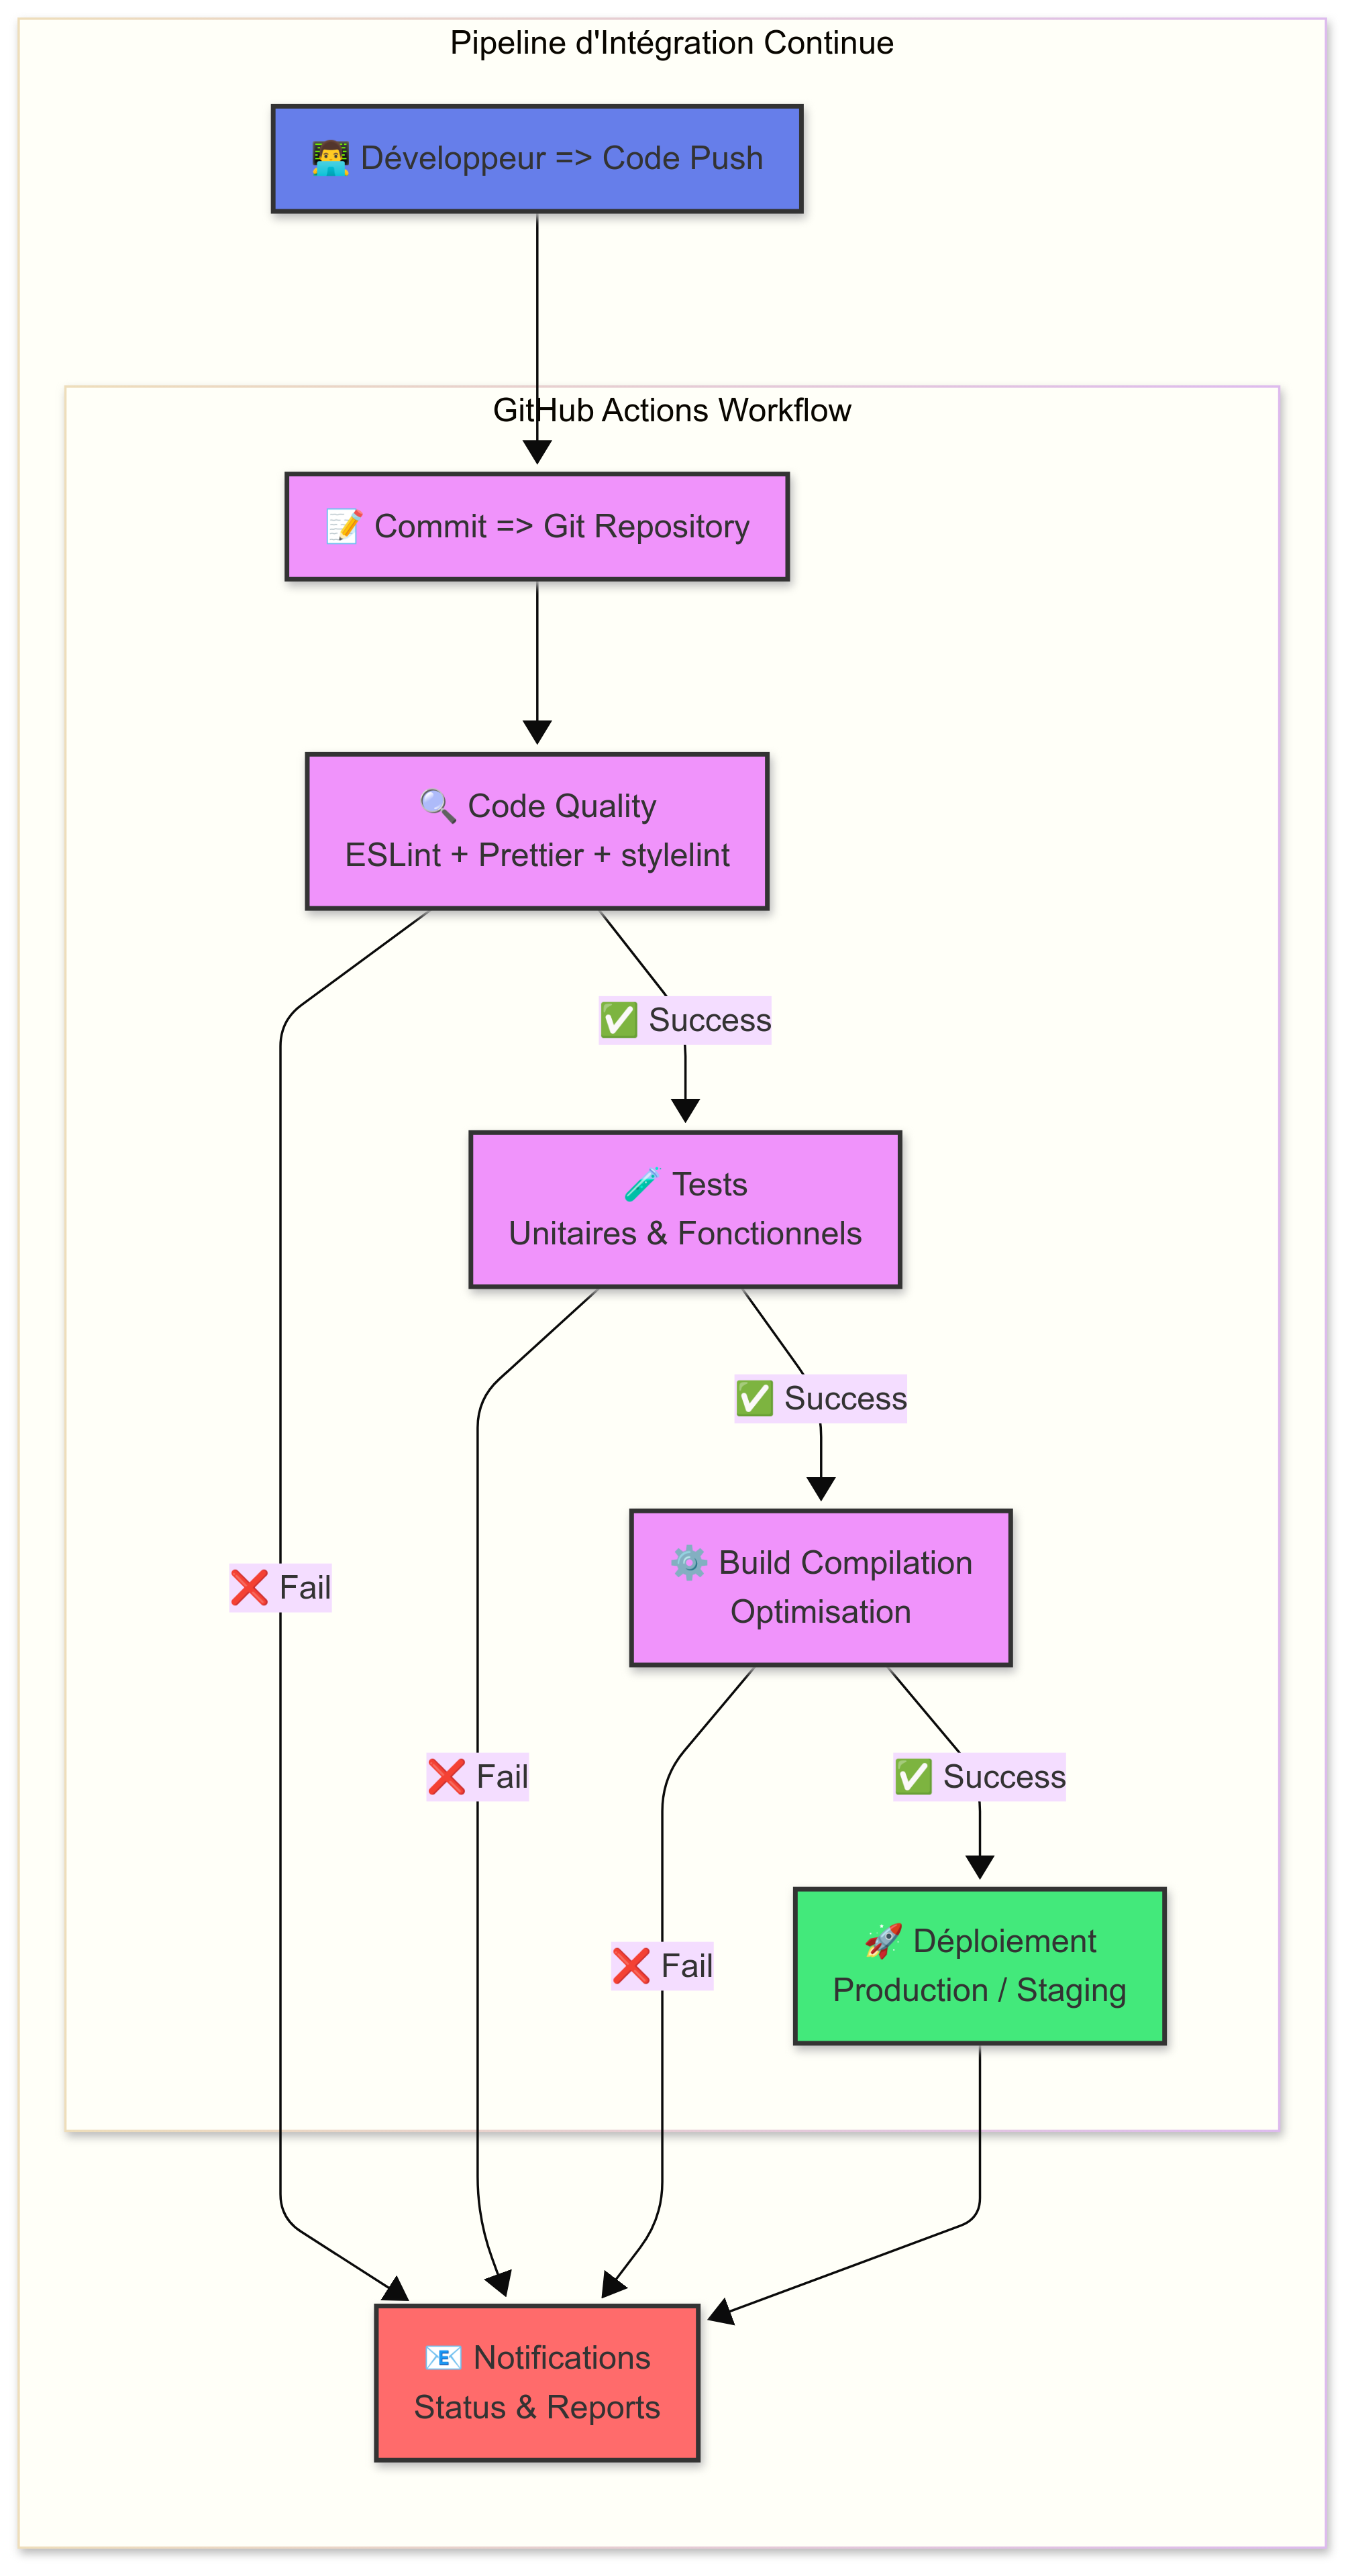
\includegraphics[width=0.8\linewidth]{pipeline.png}
\caption{Pipeline GitHub Actions automatisé}
\label{fig:cicd-pipeline}
\end{figure}

\subsection{Release automation}
Gestion sémantique des versions avec \texttt{release-it} :
\begin{itemize}
\item \textbf{Changelog} : Génération automatique
\item \textbf{Versioning} : Respect de SemVer
\item \textbf{GitHub Releases} : Publication automatisée
\end{itemize}

%------------------------------------------------------------
\section{Architecture de déploiement}

\subsection{Infrastructure de production}

L'architecture de déploiement du LMS Didier privilégie la haute disponibilité et la performance
pour répondre aux exigences critiques des fiduciaires belges. Notre infrastructure est conçue pour
supporter une montée en charge progressive tout en maintenant une qualité de service optimale.

\begin{figure}[htbp]
\centering
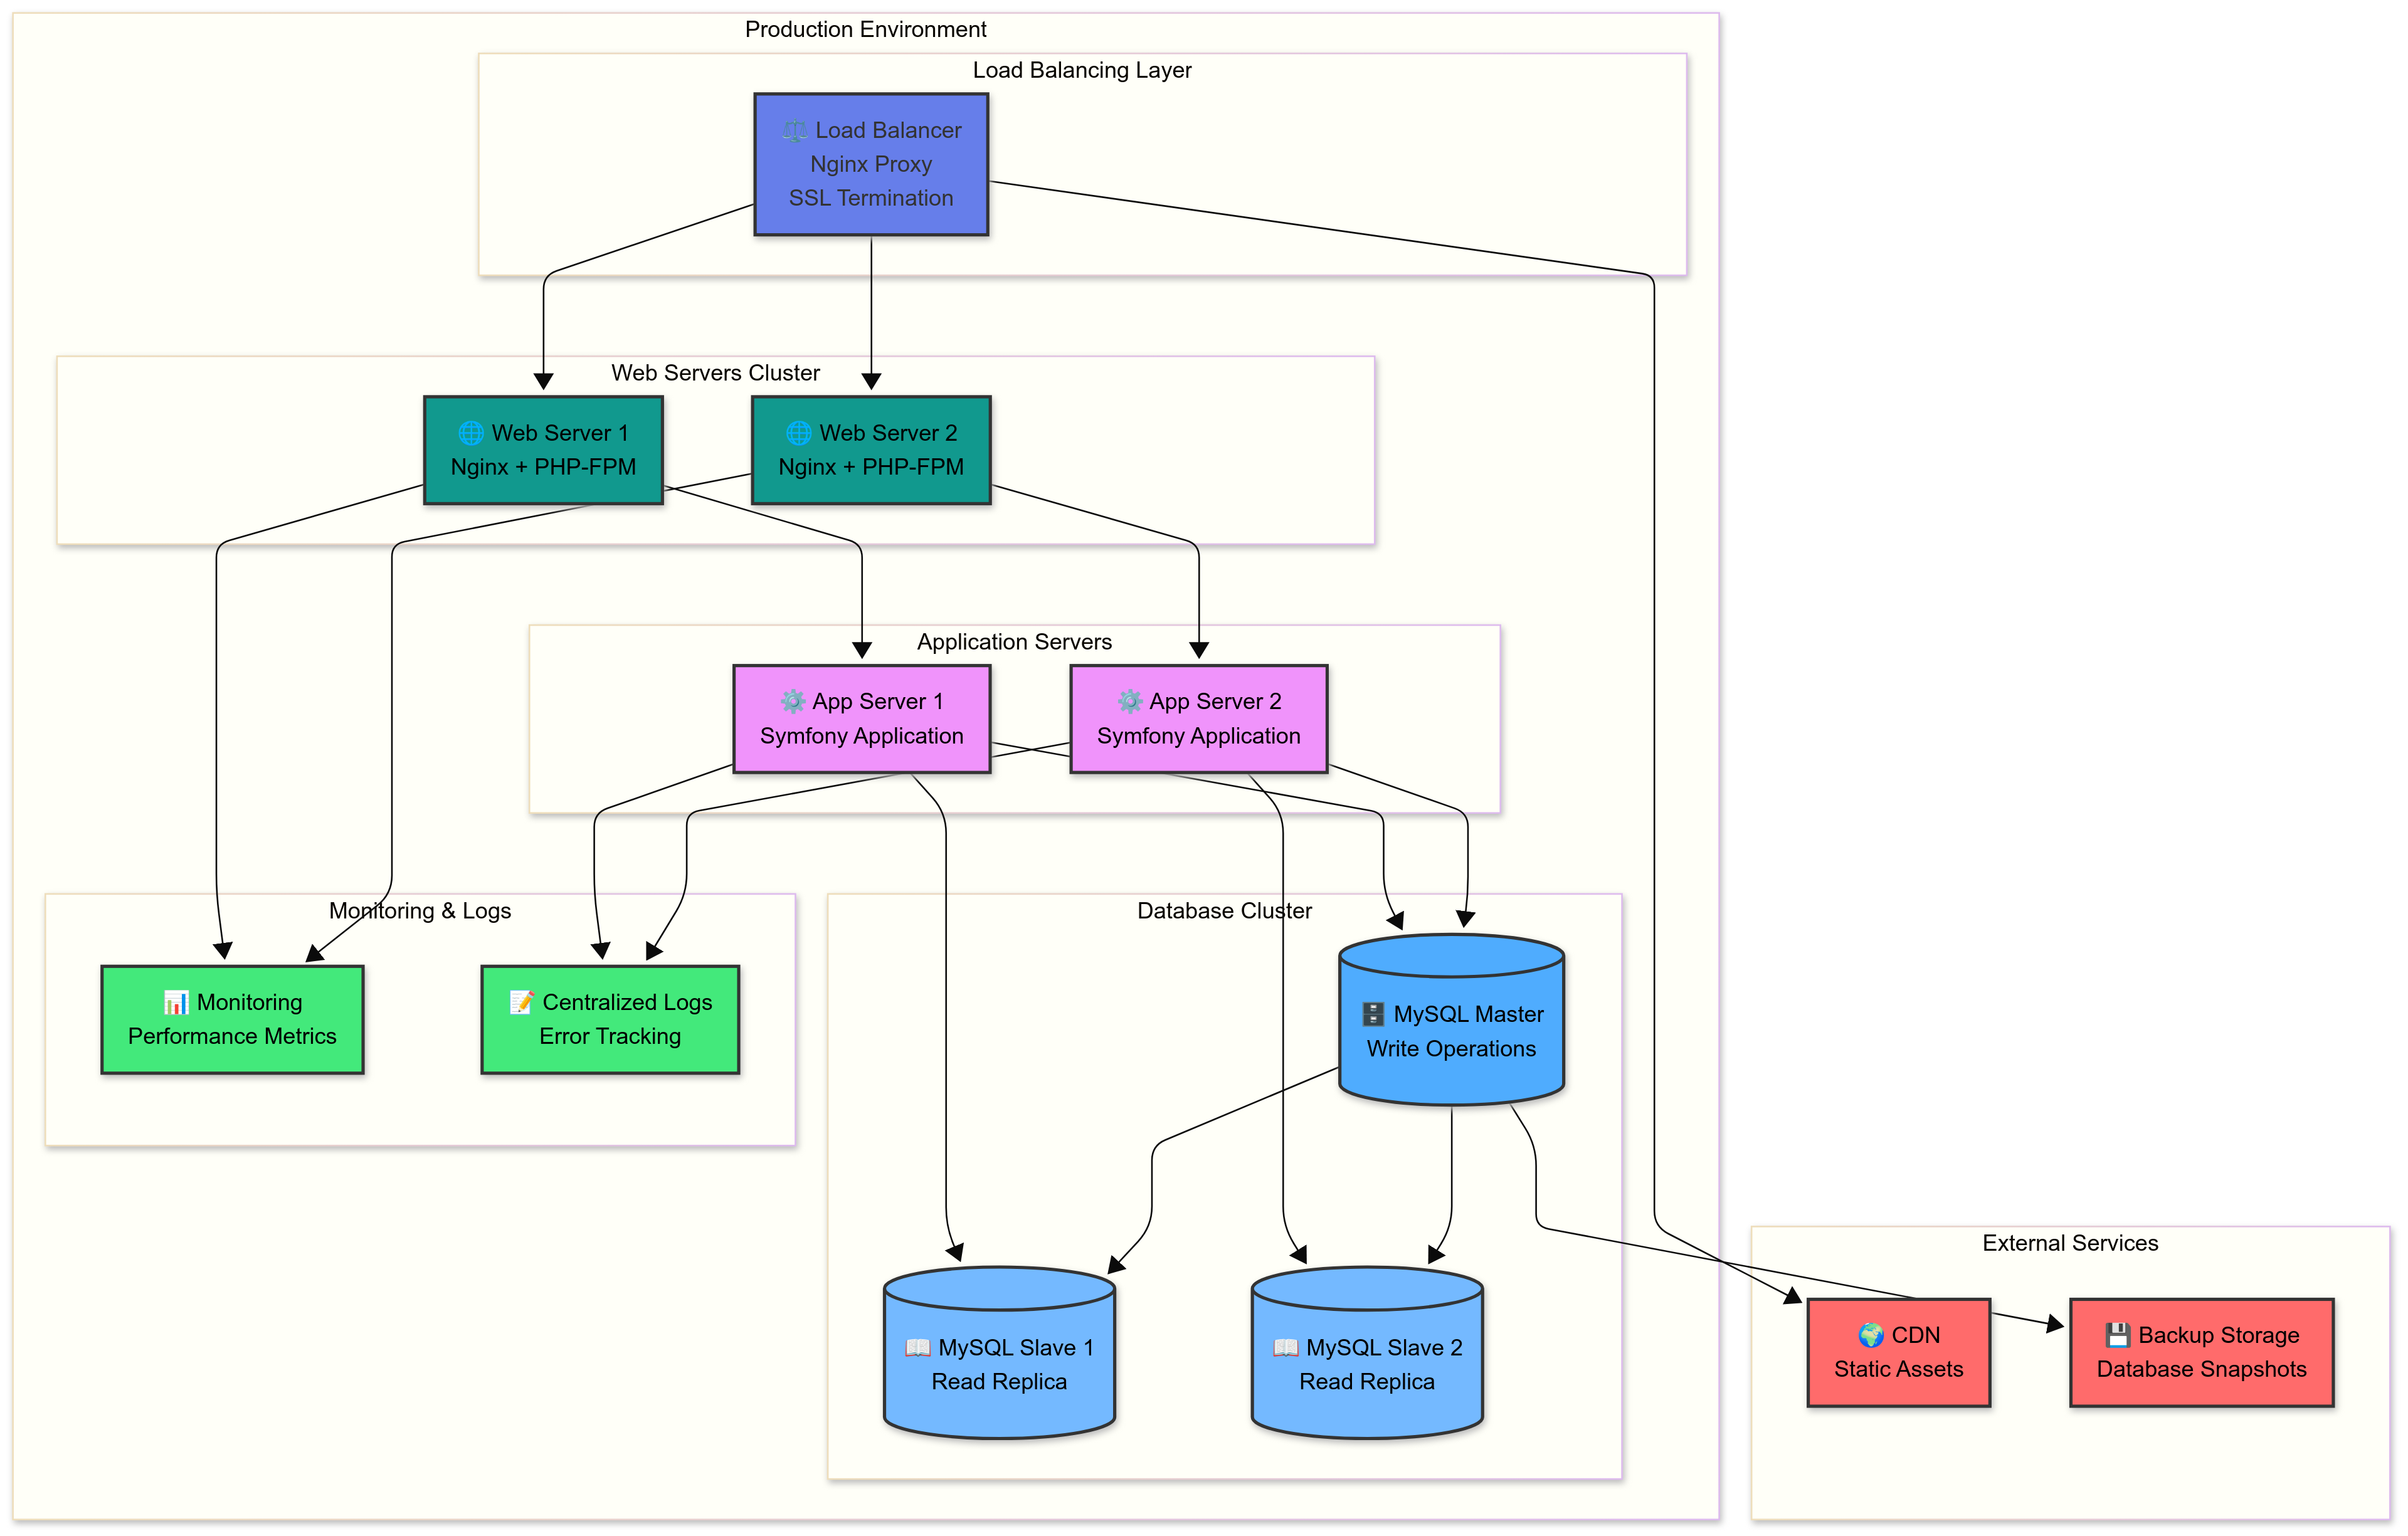
\includegraphics[width=1.0\linewidth]{Chapters/production.png}
\caption{Architecture de déploiement haute disponibilité}
\label{fig:deployment-arch}
\end{figure}

\subsection{Caractéristiques de l'infrastructure}
\begin{itemize}
\item \textbf{Haute disponibilité} : Redondance à tous les niveaux pour éliminer les points de défaillance unique
\item \textbf{Scalabilité horizontale} : Ajout transparent de serveurs selon la charge
\item \textbf{Répartition de charge} : Distribution intelligente du trafic via Nginx
\item \textbf{Base de données distribuée} : Configuration Master/Slave pour optimiser les performances lecture/écriture
\item \textbf{Monitoring continu} : Surveillance proactive des métriques de performance
\item \textbf{Sauvegarde automatisée} : Protection des données critiques avec snapshots réguliers
\end{itemize}

%------------------------------------------------------------
\section{Conclusion}
L'architecture technique du projet TT Webinar combine performance et maintenabilité grâce à des choix
technologiques éprouvés et une infrastructure moderne. Les diagrammes présentés illustrent la robustesse
de notre approche, depuis l'architecture physique jusqu'au déploiement en production. Les outils de qualité
et d'intégration continue garantissent la pérennité du code, tandis que l'architecture de déploiement assure
une disponibilité optimale pour les utilisateurs finaux. Le chapitre suivant détaillera les aspects spécifiques
d'implémentation du projet TT Webinar.